%% Desarrollo PSO velocidad

\chapter{PSO para la velocidad del viento en Valparaíso}
En este capítulo se presenta la implementación de la técnica \emph{Particle Swarm Optimization} basada principalmente en el trabajo de Carneiro et al. \cite{Carneiro15}. En principio se definen y explican los principales conceptos para entender la solución propuesta, para luego mostrar los resultados obtenidos al buscar los parámetros de ajuste de la distribución de Weibull.

\section{Modelo Matemático} \label{ss:Modelo_Mat}
Como se mencionó anteriormente, para encontrar los parámetros de la distribución de Weibull que se ajusten a los datos de prueba se utilizará la meta-heurística \emph{Particle Swarm Optimization}. La función de distribución de Weibull está definida en la ecuación \ref{eq:weibull}. La función objetivo se describe con la fórmula \ref{eq:PSO_FO} y es aquella con la que se busca minimizar el error cuadrático entre la frecuencia real de los datos y la estimada por la distribución de Weibull. Los parámetros a encontrar $k$ y $c$ deben ser $\geq 0$. Para encontrar estos parámetros se construyó el PSO que se detalla a continuación.

\section{Estructura del PSO}
Es esta sección se detallará cada una de los componentes del algoritmo, destacando algunas consideraciones importantes para el correcto desempeño de este método.
\subsection{Representación}
Cada vector posición de las partículas del enjambre representa una solución candidata la cual varía dentro de cierto espacio de búsqueda definido por los límites de las componentes. Así, para el caso de los parámetros de la distribución de Weibull, la posición de las partículas está representada por los parámetros $k$ y $c$ quedando de la forma:
\begin{align}
    x = (k, c)
\end{align}    
Para ambos parámetros, se establecen los límites entre $0.00 \leq (k,c) \leq 20.00$; criterio que se basa en el trabajo de Carneiro et al. \cite{Carneiro15}. De esta forma, las partículas se moverán dentro de ese rango, manteniéndose en los lugares que minimizan la función objetivo, la cual representa el error de la predicción de Weibull versus los datos reales.\\
Así, para cada partícula se define una estructura que posee las siguientes propiedades: 
\begin{enumerate}\label{rep:Particle}
    \item Posición: vector de largo dos de números flotantes, los cuales representan la ubicación de la partícula dentro del espacio de búsqueda y sus componentes a los parámetros $k$ y $c$.
    \item Velocidad: vector de números flotantes que representan el cambio de valor de cada componente de la posición de la partícula en determinada iteración. Se actualiza en base a la ecuación de velocidad del PSO:
    \begin{align}\label{eq:PSO}
      v_{i,j}^{k+1} &= wv_{i,j}^{k} + c_{1}r_{1}(xbest_{i,j}^k - x_{i,j}^k) + c_{2}r_{2}(xgbest_{j}^{k} - x_{i,j}^k)
    \end{align} 
    En donde $v_{i,j}^{k+1}$ es la velocidad de la partícula en el instante $k+1$, $w$, $c_1$ y $c_2$ son los parámetros de inercia, cognitivo y social respectivamente, $r_{1}$ y $r_{2}$ son números aleatorios entre $[0, 1]$, $xbest_{i,j}^k$ y $xgbest_{j}^{k}$ son la mejor solución de la partícula y la mejor solución del vecindario respectivamente en el instante $k$, $x_{i,j}^k$ representa la posición de la partícula, o la solución, en el instante $k$.    
    \item Mejor resultado personal: vector flotante que guarda la mejor posición conseguida por la partícula durante las iteraciones transcurridas.    
\end{enumerate}        
Mientras que el enjambre, siendo esencialmente una estructura que posee referencia a todas las partículas, queda representado de la siguiente forma:
\begin{enumerate}\label{rep:Swarm}
    \item Partículas: Arreglo de referencias a las estructuras de partículas creadas.
    \item Mejor posición global: De todos los mejores resultados de cada partícula, se almacena la mejor posición de todas. La que persiste al final del ciclo de iteraciones, es la solución final.
\end{enumerate} 

%% Ajustar para que sea coherente
\subsection{Consideración de los parámetros}
Los parámetros $w$ de inercia, $c_1$ cognitivo y $c_2$ social del PSO determinan con qué peso inciden en el camino que siguen las partículas del enjambre, la velocidad anterior, la solución particular y la solución global respectivamente.\\ 
La inercia $w$ regula qué magnitud de la velocidad anterior se mantiene en la actual, así la partícula se comporta similar a un cuerpo desacelerando. En Kaveh \cite{Psoexplain14} se explica que en términos extremos, si la velocidad previa se elimina (peso nulo), las partículas no pueden salir del círculo local relativo a las soluciones iniciales, lo que sería equivalente a un procedimiento de búsqueda local.  Por el contrario, si se le da mucho peso, las partículas tenderían a huir de las buenas posiciones conocidas.\\
El parámetro cognitivo $c_1$ controla la influencia de la mejor solución encontrada por la partícula misma en la velocidad actual. Si se le da un peso mayor a este valor, la partícula tenderá a explorar las zonas locales a la posición desde donde partió.\\
El parámetro social $c_2$ controla la influencia de la mejor solución global encontrada por el enjambre en la velocidad actual. Si se le da un peso mayor a este valor, la partícula tenderá a explotar las zonas locales a la posición de la solución global.\\
La convergencia prematura es un comportamiento presente en el \emph{Particle Swarm Optimization}, como se explica nuevamente en Kaveh \cite{Psoexplain14}. Esto se debe a que normalmente, las partículas se concentran en una ``nube'' local a la mejor solución global una vez que se ha avanzado ciertas iteraciones, lo que por una lado hace que el algoritmo sea más rápido que otras técnicas afines, como los algoritmos evolutivos, pero por otro impide que, a partir de cierto punto, se siga mejorando la solución. Por tanto, hay un límite óptimo para las iteraciones, ya que en cierto momento las partículas se quedarán atrapadas en un óptimo local.\\
A modo de evitar la convergencia prematura, varias técnicas han sido propuestas, las cuales se resumen en el trabajo de Kaveh \cite{Psoexplain14}. Para esta memoria, se utilizará la recomendación de Chang \cite{Chang10_2} para la variación de parámetros del enjambre:
\begin{align}\label{eq:VariationParameters}
    w(j) &= (1 - \frac{j}{iter_{max}})^{\alpha}(w_{max} - w_{min}) + w_{min}\\
    c_{1}(j) &= (1 - \frac{j}{iter_{max}})^{\beta}(c_{1max} - c_{1min}) + c_{1min}\\
    c_{2}(j) &= (1 - \frac{j}{iter_{max}})^{\gamma}(c_{2min} - c_{2max}) + c_{2max}
\end{align}    
Donde $w(j)$, $c_{1}(j)$, $c_{2}(j)$, son los parámetros de inercia, cognitivo y social en el instante $j$. Los valores para los rangos de los parámetros son $w_{max} = 0.9$ y $w_{min} = 0.4$, $c_{1max}$, $c_{2max}$ y $c_{1min}$, $c_{2min}$, 2.5 y 0 respectivamente. Los parámetros $\alpha, \beta, \gamma$ son definidos como 0.5, 1.5 y 1.0 respectivamente. La variable $iter_{max}$ es el máximo número de iteraciones. \\
Esta modificación provocará que las partículas ``frenen'' su convergencia al óptimo local, dado que en cada iteración se da menos peso a la solución global y mayor peso al óptimo de cada partícula y a la velocidad anterior.

\subsection{Descripción del algoritmo}
La estructura del PSO se detalla en el Algoritmo \ref{alg:pso}. Este se basa en mover las partículas dentro del rango definido para los componentes de la solución hasta que todas las partículas se concentren en alguna zona que represente una buena solución al problema, no necesariamente el óptimo. Lo importante en cada iteración es actualizar o mover el enjambre, revisar y guardar las mejores soluciones y actualizar los parámetros de inercia, cognitivo y social que definen las velocidades.
%!TEX root = main.tex

\begin{algorithm}[h!]
\caption{PSO para el ajuste de los parámetros de la distribución de Weibull}
\label{alg:pso}
\begin{algorithmic}
\REQUIRE Datos de frecuencias de velocidades del viento.
\ENSURE Valores para los parámetros $k$ y $c$.
\STATE enjambre = inicializar(w,c1,c2)
\FOR{$i = 1$ to $Iter_{max}$}
\FOR{Each partículas en enjambre}
    \STATE actualizarVelocidadPartícula(partícula)
    \STATE actualizarPosiciónPartícula(partítucla)
    \STATE guardarMejorResultadoPartícula(partícula)
\ENDFOR
\STATE guardarMejorResultadoGlobal(enjambre)
\STATE actualizarParámetros(enjambre)
\ENDFOR
\STATE retornarMejorResultadoGlobal(enjambre).
\end{algorithmic}
\end{algorithm}

\section{Resultados}\label{sec:Experimentos_velocidad}
En esta sección se presentan los resultados obtenidos en los experimentos realizados para el ajuste de la distribución de Weibull a diferentes conjuntos de datos del viento en Valparaíso.
\subsection{Experimentos}
Los experimentos fueron probados hasta en un máximo de 1000 iteraciones y 50 partículas, (A excepción del experimento donde se consideraron todos los promedios diarios, 2013, 2014 y 2015, en el cual, se utilizaron 200 partículas). \\
Con el fin de evitar que los resultados estén sesgados por el azar, dado los factores aleatorios presentes en la fórmula del PSO 
\ref{rep:Swarm}, se repiten los experimentos realizados 30 veces cambiando la semilla generadora de números aleatorios. \\
Los parámetros de $w$, $c1$ y $c2$ fueron definidos tal y como explica en el modelo matemático, en la sección \ref{ss:Modelo_Mat}.\\
Los experimentos fueron realizados con datos del viento obtenidos por la Armada de Chile para la región de Valparaíso en los años 2013, 2014 y 2015. Estos fueron tratados mediante \emph{scripts} desarrollados en \emph{Python} para obtener las frecuencias de las distintas velocidades del viento registradas a lo largo del año. Los datos se organizaban de la siguiente forma: Por cada año, se tiene una tabla en un archivo excel de cada mes, en donde se registra por cada fila los resultados de la medición de cada día. Las mediciones son registradas en un intervalo de tres horas, es decir, se tienen registros diarios para las 3:00, 6:00, 9:00, 12:00, 15:00, 18:00, 21:00 y 00:00 horas. Un ejemplo es la tabla mostrada en la Figura \ref{fig:example_data}.\\
 \begin{figure}[h!]
    \centering
    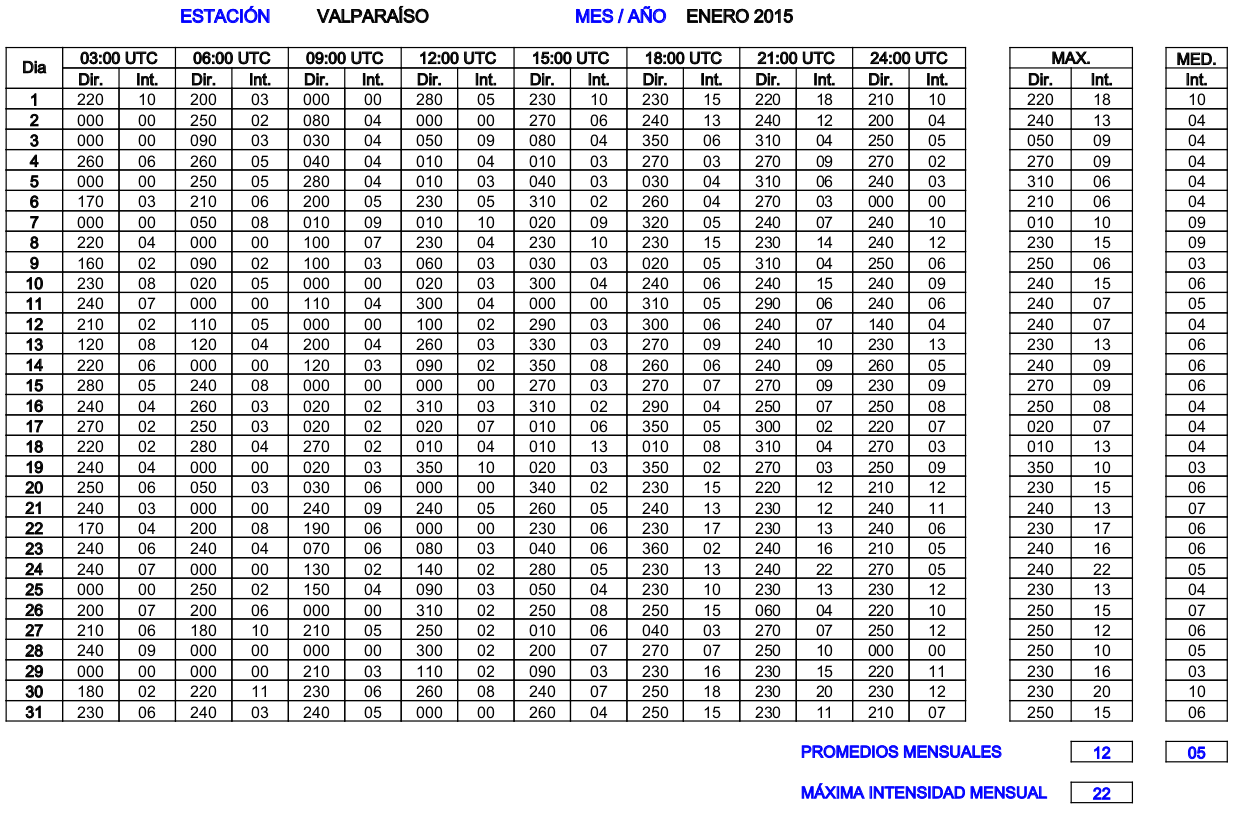
\includegraphics[height=100mm]{figures/example_data.png}
    \caption{Ejemplo colección de datos Enero Valparaíso 2015}
    \vspace{-.25cm}
    \caption*{Fuente: Instituto Meteorológico de la Armada de Chile.}
    \label{fig:example_data}
 \end{figure}
El ajuste de la distribución de Weibull a estos datos de velocidad del viento se hizo considerando las siguientes configuraciones para el cálculo del
histograma de frecuencias:
\begin{enumerate}
\item \textbf{Anual}. Se considera el promedio diario de velocidad del viento como dato unitario para el cálculo de las frecuencias en
  un lapso anual (2013, 2014 y 2015).
  \item \textbf{Todos los años}. Se considera el promedio diario de velocidad del viento como dato unitario para el cálculo de las frecuencias, considerando
  todos los días en el intervalo de Enero del 2013 hasta Diciembre del 2015.
  \item \textbf{Por temporada}. Se considera el promedio diario de velocidad del viento como dato unitario para el cálculo de las frecuencias en
  un lapso de tres meses (Enero - Marzo ; Abril - Junio; Julio - Septiembre; Octubre - Diciembre).
  \item \textbf{Datos brutos}. Se considera cada medición realizada (8 por día) como dato unitario, en un lapso de un año (2015).
\end{enumerate}

Una vez obtenidos los datos de frecuencias, se procede a aplicar el algoritmo \emph{Particle Swarm Optimization} donde se obtienen los parámetros de ajuste $k$ y $c$. De esta manera, se evalúa la calidad del modelo generado (distribución de densidad de probabilidad de Weibull), para las distintas configuraciones mediante gráficos y los siguientes test estadísticos (utilizados también en el trabajo de Carneiro et al. \cite{Carneiro15}):
\begin{enumerate}
    \item \emph{Root Mean Square Error}
        \begin{align}
            RMSE = \sqrt{\frac{\sum_{i=1}^{N}(X_i - Y_i)^2}{N}}
        \end{align}    
    \item \emph{Correlation}
        \begin{align}
            r = \frac{\sum_{i=1}^{N}(X_i - X_{med})\cdot(Y_i - Y_{med})}{\sqrt{\sum_{i=1}^{N}(X_i - X_{med})^2}\cdot\sqrt{\sum_{i=1}^{N}(Y_i - Y_{med})^2}}
        \end{align}    
    \item \emph{Relative Bias}
        \begin{align}
            RB = \frac{X_{med} - Y_{med}}{Y_{med}}  
        \end{align}    
\end{enumerate}        
Donde $N$ es el número de datos, $Y_i$ la frecuencia de dichos datos, $X_i$ la frecuencia entregada por la distribución de Weibull, $X_{med}$ la media de $X_i$ e $Y_{med}$ la media de $Y_i$. \\

Las pruebas fueron realizadas en un computador con sistema operativo Ubuntu 16.04 64-bit, 3.8 GB de memoria y procesador doble núcleo Intel Pentium 2.60 GHz. 

\subsection{Análisis de los resultados}
\subsubsection{Visualización de los datos}
Los gráficos \ref{fig:data_valpo_13}, \ref{fig:data_valpo_14} y \ref{fig:data_valpo_15} muestran la distribución de datos de velocidad del viento en Valparaíso a lo largo de los meses del año y las horas del día, lo cual permite visualizar la naturaleza de la intensidad del viento de forma cualitativa.
Por ejemplo, se logra apreciar que las máximas velocidades son obtenidas en los meses finales de primavera y comienzos de verano.\\
Las superficies que se exponen no representan la distribución continua de los datos. Estos fueron graficados de forma discreta y posteriormente la herramienta utilizada para generar la superficie unió los puntos mediante rectas.\\
\begin{figure}[ht!]
     \centering
     \captionsetup{justification=centering,margin=2cm}
        \subfigure[Vientos Valparaíso 2013.]{
            \label{fig:data_valpo_13}
            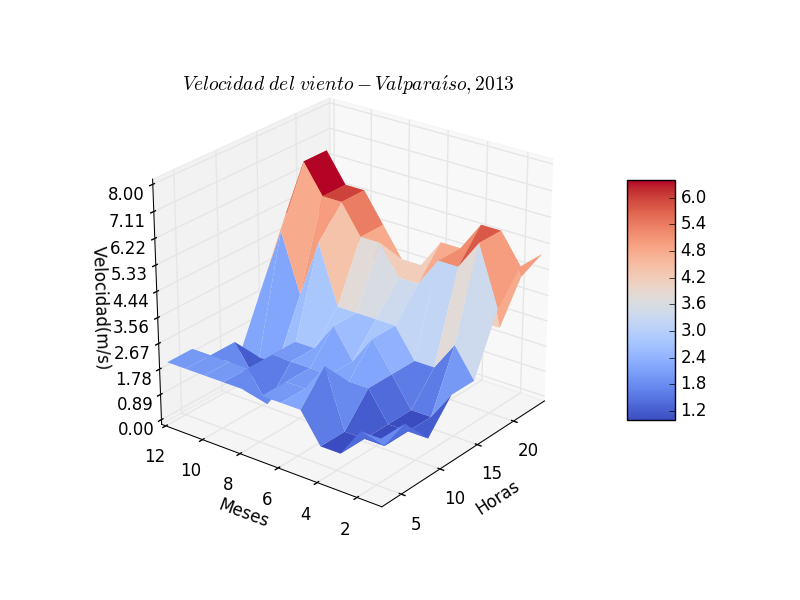
\includegraphics[width=0.45\textwidth]{figures/3d_data_2013.png}
        }%
         \subfigure[Vientos Valparaíso 2014.]{
            \label{fig:data_valpo_14}
            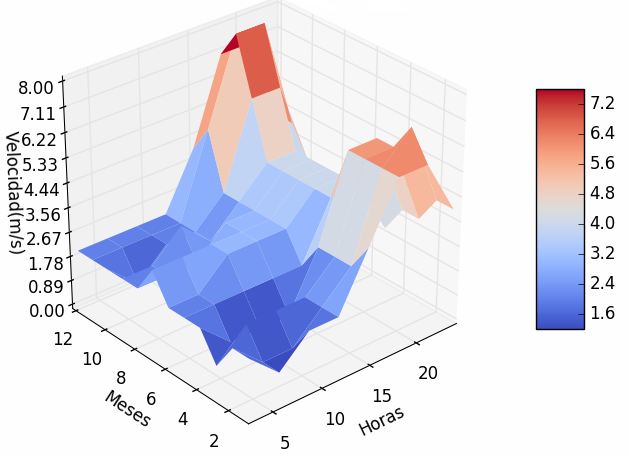
\includegraphics[width=0.45\textwidth]{figures/3d_data_2014.png}
        }\\
         \subfigure[Vientos Valparaíso 2015.]{
            \label{fig:data_valpo_15}
            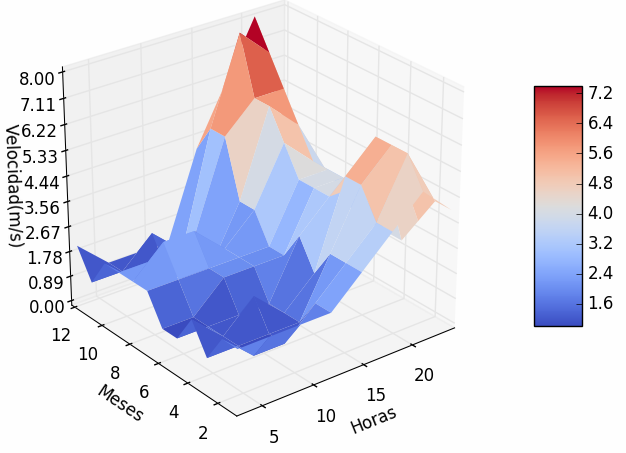
\includegraphics[width=0.45\textwidth]{figures/3d_data_2015.png}
        }%
    \caption{Superficie de datos viento de Valparaíso.}
    \caption*{Fuente: Elaboración Propia.}
    \label{fig:subfigures}
\end{figure}

\subsubsection{Experimento 1, datos anuales y promedios diarios}
Las figuras \ref{fig:pso_valpo_13}, \ref{fig:pso_valpo_14} y \ref{fig:pso_valpo_15} muestran el ajuste de la distribución de Weibull a los histogramas de datos del viento (promedios diarios), con los parámetros $k$ y $c$  que se muestran en las primeras tres filas de la tabla \ref{table:stadistical_tests} determinados por el PSO. El ajuste tiene buena forma, lo cual es corroborado por los datos estadísticos obtenidos con los test previamente mencionados (RMSE, r, RB), expuestos en la tabla \ref{table:stadistical_tests} en las filas 1, 2 y 3. Si se compara con la precisión conseguida en el trabajo de Carneiro et al. \cite{Carneiro15}, se aprecia que el ajuste conseguido es levemente más impreciso, sobre todo en lo relativo al test \emph{relative bias} (RB) el cual es una medida de distancia de la frecuencia estimada con la de los datos. Esto podría deberse a la naturaleza de los datos 
trabajados.\\
\begin{figure}[ht!]
    \centering
    \captionsetup{justification=centering,margin=2cm}
        \subfigure[PSO Valparaíso 2013.]{
            \label{fig:pso_valpo_13}
            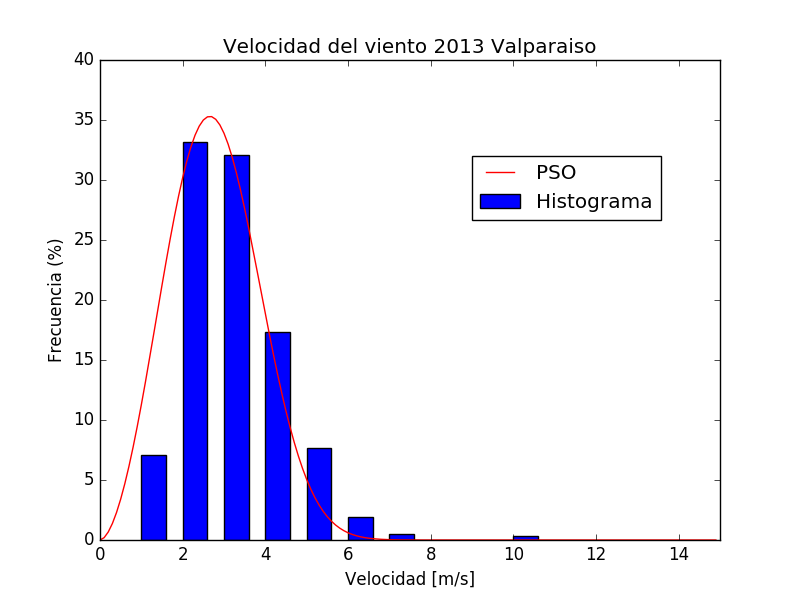
\includegraphics[width=0.45\textwidth]{figures/result_2013.png}
        }%
        \subfigure[PSO Valparaíso 2014.]{
            \label{fig:pso_valpo_14}
            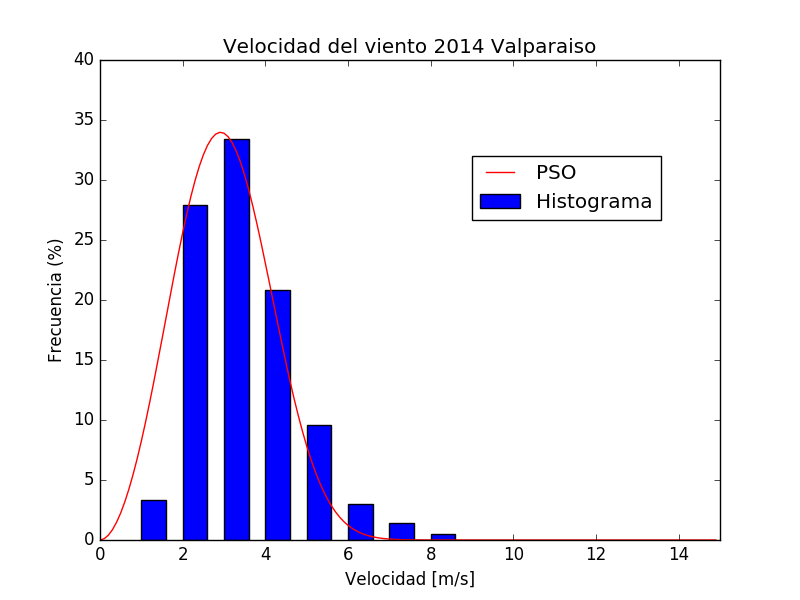
\includegraphics[width=0.45\textwidth]{figures/result_2014.png}
        }\\
        \subfigure[PSO Valparaíso 2015.]{
            \label{fig:pso_valpo_15}
            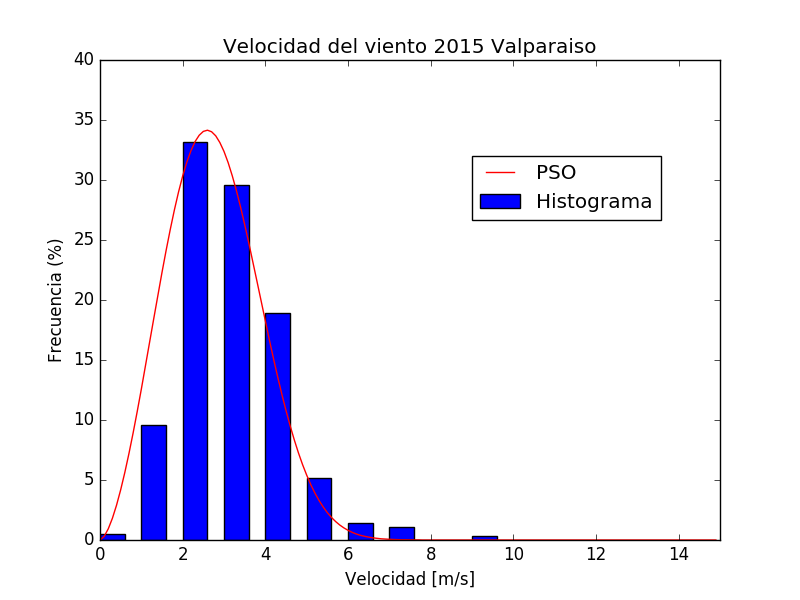
\includegraphics[width=0.45\textwidth]{figures/result_2015.png}
        }%
    \caption{Ajuste con PSO a datos del viento de Valparaíso.}
    \caption*{Fuente: Elaboración Propia.}
    \label{fig:subfigures}
\end{figure}

\subsubsection{Experimento 2, datos de tres años en conjunto y promedios diarios}
En este experimento se realizó el ajuste considerando los promedios diarios y un intervalo de tres años consecutivos. El gráfico \ref{fig:pso_valpo_15_14_13_lq}, muestra el resultado del ajuste con PSO y la configuración estándar de los experimentos, es decir, 100 iteraciones y 50 partículas. En este gráfico se aprecia que el ajuste no es bueno, a pesar de las cifras en la tabla \ref{table:stadistical_tests}, fila 4: PSO (50p), dado que oscila bastante alrededor de las barras del histograma, por lo que se repite el experimento aumentando el número de partículas a 200 obteniendo el gráfico \ref{fig:pso_valpo_15_14_13}, con el cual se obtiene un ajuste más adecuado, además de mejorar los resultados de los test estadísticos (tabla \ref{table:stadistical_tests}, fila 5: PSO (200p)).\\
\begin{figure}[ht!]
    \centering
    \captionsetup{justification=centering,margin=2cm}
        \subfigure[Buen ajuste PSO Valparaíso 2013.]{
            \label{fig:pso_valpo_15_14_13}
            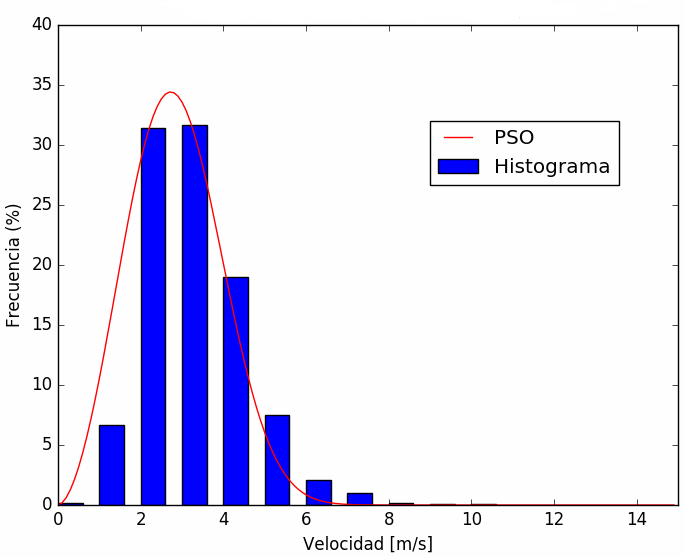
\includegraphics[width=0.45\textwidth]{figures/result_13-14-15.png}
        }%
        \subfigure[Mal ajuste PSO Valparaíso 2013.]{
            \label{fig:pso_valpo_15_14_13_lq}
            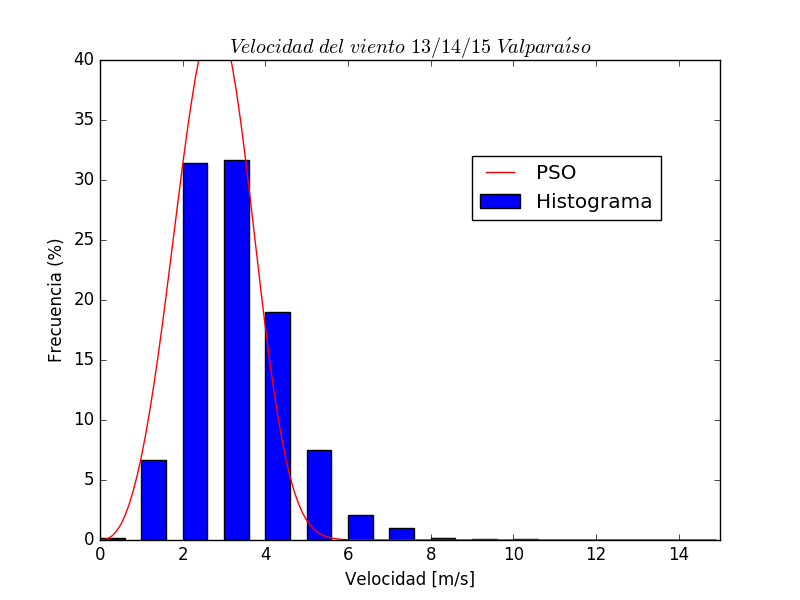
\includegraphics[width=0.45\textwidth]{figures/result_13-14-15_low_quality.png}
        }%
    \caption{Ajuste con PSO a datos Valparaíso 2015, 2014 y 2013, baja y buena calidad.}
    \caption*{Fuente: Elaboración Propia.}
    \label{fig:subfigures}
\end{figure}

\subsubsection{Experimento 3, ajuste a datos anuales con resultados del experimento 2}
Los gráficos \ref{fig:pso_valpo_13_all_data}, \ref{fig:pso_valpo_14_all_data} y \ref{fig:pso_valpo_15_all_data} son ajustes de Weibull con los parámetros obtenidos en el experimento anterior. Es decir, la idea es evaluar el modelo general de los tres años versus el histograma de datos de cada año en particular.
El ajuste desde los resultados estadísticos (tabla \ref{table:stadistical_tests}), es levemente menos preciso que el modelo ajustado a cada año en particular, pero sigue siendo aceptable como posible opción a considerar.
\begin{figure}[ht!]
    \centering
    \captionsetup{justification=centering,margin=2cm}
    \subfigure[Velocidad viento Valparaíso 2013.]{
        \label{fig:pso_valpo_13_all_data}
        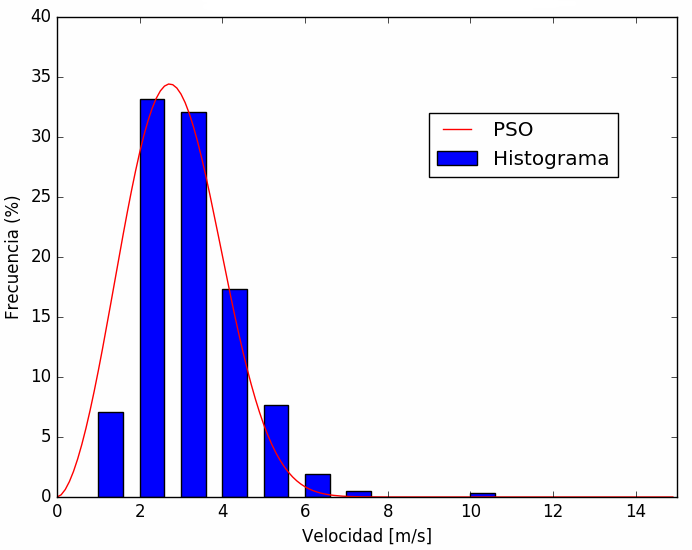
\includegraphics[width=0.45\textwidth]{figures/result_2013_fit_all_data.png}
    }%  
    \subfigure[Velocidad viento Valparaíso 2014.]{
        \label{fig:pso_valpo_14_all_data}
        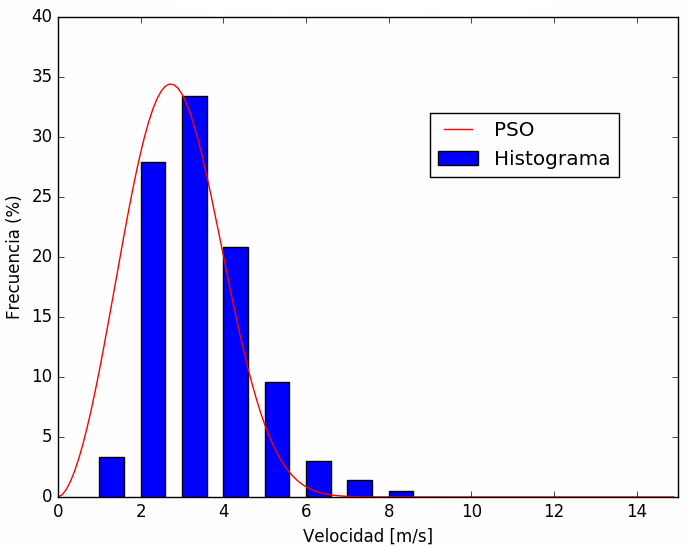
\includegraphics[width=0.45\textwidth]{figures/result_2014_fit_all_data.png}
    }\\   
    \subfigure[Velocidad viento Valparaíso 2015.]{
        \label{fig:pso_valpo_15_all_data}
        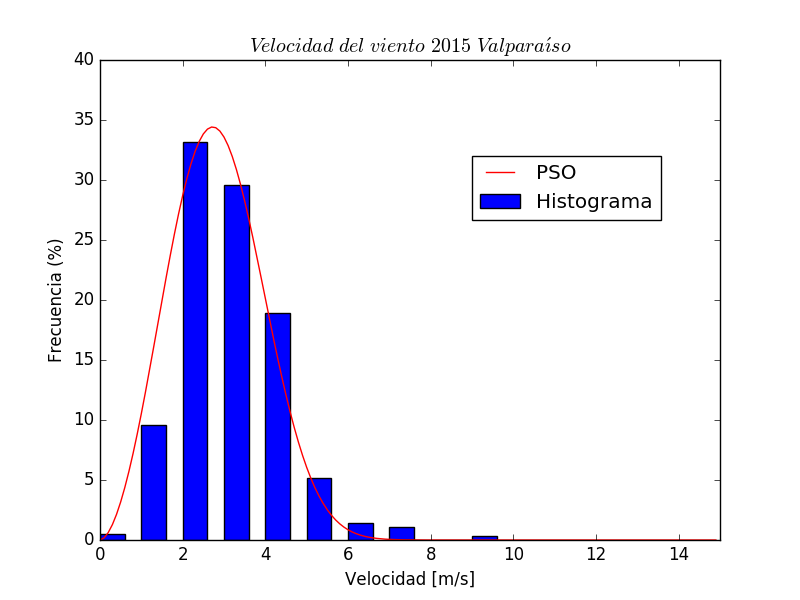
\includegraphics[width=0.45\textwidth]{figures/result_2015_fit_all_data.png}
    }%     

    \caption{Ajuste con PSO a registros del viento en Valparaíso (Con todos los datos).}
    \caption*{Fuente: Elaboración Propia.}
    \label{fig:subfigures}
\end{figure}

\subsubsection{Experimento 4, ajuste a datos de tres meses y promedios diarios}
Es posible que se requiera un análisis más acotado, por ello los gráficos \ref{fig:pso_valpo_15_ene_mar}, \ref{fig:pso_valpo_15_abr_jun}, 
\ref{fig:pso_valpo_15_jul_sep}, \ref{fig:pso_valpo_15_oct_dic}, muestran un ajuste considerando un lapso de 3 meses para el año 2015, con el
que se demuestra que es posible definir cualquier intervalo (manteniendo como unidad de dato el promedio diario de velocidad del viento)
 y obtener un ajuste adecuado de los datos mediante la distribución de Weibull.

\begin{figure}[ht!]
    \centering
    \captionsetup{justification=centering,margin=2cm}
    \subfigure[Enero - Marzo.]{
        \label{fig:pso_valpo_15_ene_mar}
        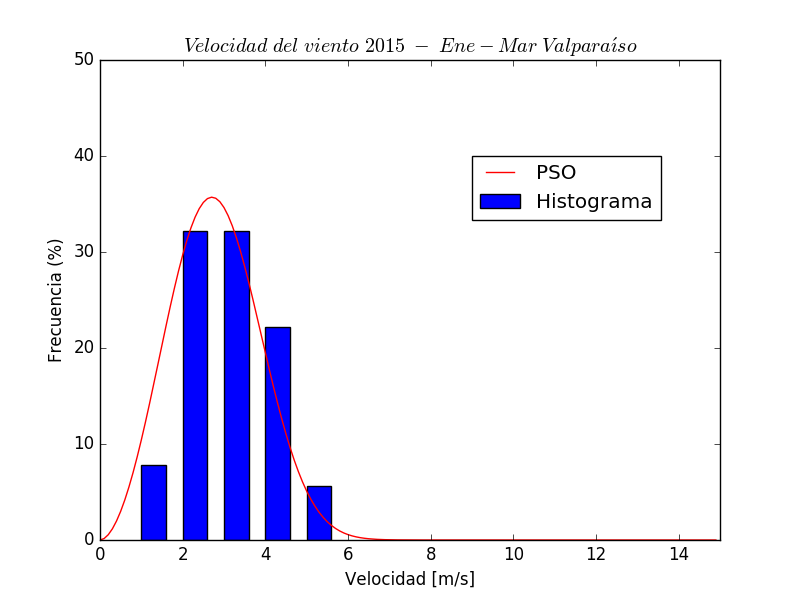
\includegraphics[width=0.45\textwidth]{figures/result_2015_Ene-Mar.png}
    }%  
    \subfigure[Abril - Junio.]{
        \label{fig:pso_valpo_15_abr_jun}
        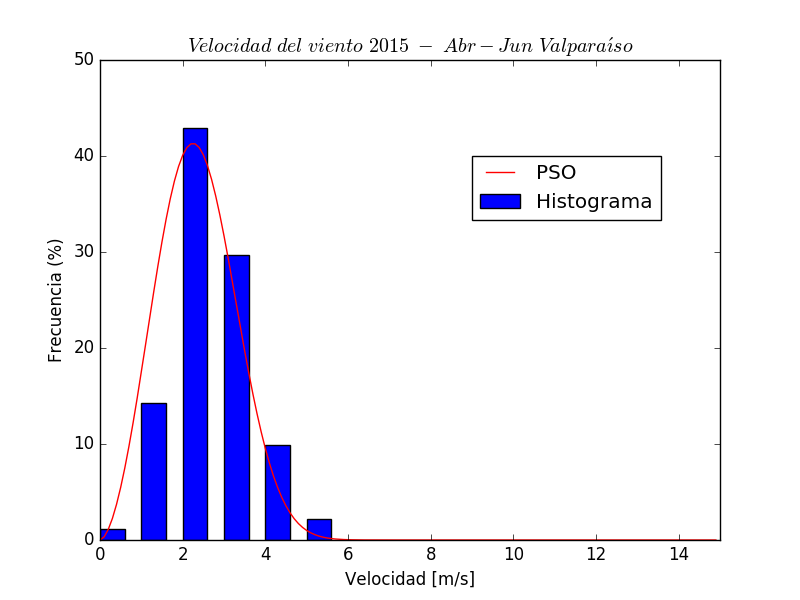
\includegraphics[width=0.45\textwidth]{figures/result_2015_Abr-Jun.png}
    }\\  
    \subfigure[Julio - Septiembre.]{
        \label{fig:pso_valpo_15_jul_sep}
        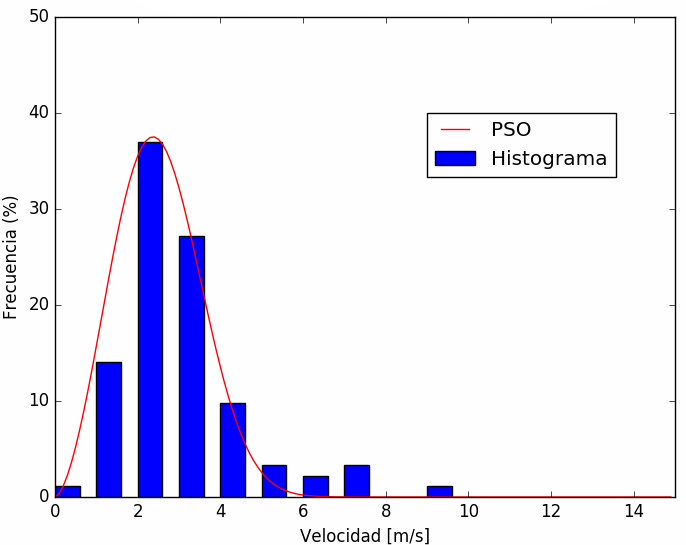
\includegraphics[width=0.45\textwidth]{figures/result_2015_Jul-Sep.png}
    }% 
    \subfigure[Octubre - Diciembre.]{
        \label{fig:pso_valpo_15_oct_dic}
        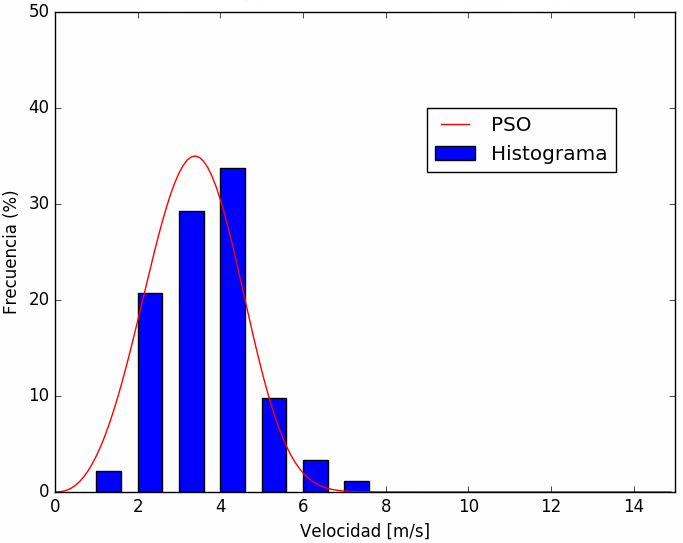
\includegraphics[width=0.45\textwidth]{figures/result_2015_Oct-Dic.png}
    }%  
    \caption{Ajuste con PSO a datos Valparaíso 2015, por rango de meses.}
    \caption*{Fuente: Elaboración Propia.}
    \label{fig:subfigures}
\end{figure}

\subsubsection{Experimento 5, ajuste a datos año 2015 y datos brutos}
La razón de por qué se utiliza el promedio diario de los datos del viento para ajustar Weibull y no las mediciones puras (las mediciones tomadas cada 3 horas diariamente) es expuesta en el gráfico \ref{fig:pso_valpo_15_all_data}. La distribución de Weibull no se ajusta a una distribución de datos con más de un máximo, por lo que de requerirse un modelo para este caso se debe buscar otra distribución o modificar la distribución de Weibull. Es por ello que normalmente se utiliza un promedio de los datos, como se realiza en el trabajo de Farade \cite{Fadare08}.
\begin{figure}[ht!]
    \centering
    \captionsetup{justification=centering,margin=2cm}
    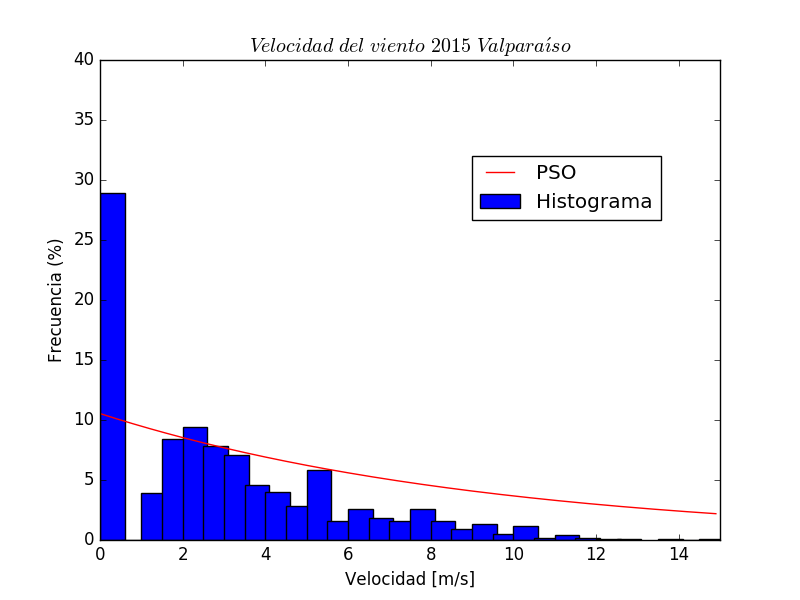
\includegraphics[width=0.45\textwidth]{figures/result_2015_all_data.png}
    \caption{Ajuste con PSO a datos (cifras puras) Valparaíso 2015, 2014, 2013}
    \vspace{-.25cm}
    \caption*{Fuente: Elaboración Propia.}
    \label{fig:pso_valpo_15_all_data}
\end{figure}
\pagebreak
\newpage
\subsubsection{Resumen de los experimentos}
En esta sección se exponen los resultados obtenidos de los experimentos realizados. En este caso la aplicación de la propuesta realizada en Carneiro et al. \cite{Carneiro15}, obtuvo los resultados esperados en cuanto a la calidad del ajuste de la distribución de Weibull a los datos del viento de Valparaíso.\\
La tabla se organiza como se explica a continuación:
\begin{enumerate}
  \item \textbf{Método}: Método utilizado para el ajuste de los parámetros de Weibull.
  \item \textbf{Periodo}: Periodo de tiempo considerado para los datos en el experimento.
  \item \textbf{k}: Parámetro $k$ de la distribución de Weibull. El valor corresponde a la mediana de las repeticiones.
  \item \textbf{c}: Parámetro $c$ de la distribución de Weibull. El valor corresponde a la mediana de las repeticiones.
  \item \textbf{RMSE}: Test estadístico conocido como \emph{root mean square error}.
  \item \textbf{r}: Test estadístico conocido como \emph{correlation}.
  \item \textbf{RB}: Test estadístico conocido como \emph{relative bias}.
  \item \textbf{Tiempo}: Tiempo total de ejecución del algoritmo.
\end{enumerate}
Los tiempos omitidos en la Tabla \ref{table:stadistical_tests}, en las filas 6, 7 y 8 indican que no se calcularon los parámetros de la función de densidad, sino que se utilizaron los obtenidos previamente, en el experimento de la fila 5. El número de iteraciones del PSO no se considera debido a que sólo se itera en la fase de desarrollo del algoritmo. Cuando este está completo, basta con una ejecución para tener el resultado definitivo del experimento.\\
En las Figuras \ref{fig:bp_param_K} y \ref{fig:bp_param_C}, se puede observar la distribución de los parámetros $k$ y $c$ obtenidos en las repeticiones de los experimentos, demostrando que independiente de la semilla de números aleatorios utilizada los resultados obtenidos son similares. La tabla \ref{table:restarts_pso_velocity} expone un resumen de las repeticiones del PSO.
\begin{table}[ht!]
    %\centering
    \caption{Tabla de pruebas, PSO velocidad del viento}
    \label{table:stadistical_tests}
    \resizebox{\textwidth}{!}{
    \begin{tabular}{|c|c|c|c|c|c|c|c|c|}
        \hline
        \textbf{\#} & \textbf{Método} & \textbf{Periodo} & \textbf{k} & \textbf{c} & \textbf{RMSE} & \textbf{r} & \textbf{RB} & \textbf{Tiempo}\\
        \hline
        1   & PSO                 & 2013        & 2.78 & 3.12                   & 2.26$\cdot 10^{-2}$ & 0.984  & 1.98$\cdot 10^{-3}$  & 1.74s\\
        2   & PSO                 & 2014        & 2.91 & 3.37                   & 2.32$\cdot 10^{-2}$ & 0.982  & 7.54$\cdot 10^{-4}$  & 1.63s\\
        3   & PSO                 & 2015        & 2.65 & 3.10                   & 1.64$\cdot 10^{-2}$ & 0.992  & 3.02$\cdot 10^{-3}$  & 1.59s\\
        \hline
        4   & PSO (50p)           & 2015-14-13  & 3.47 & 3.07                   & 3.61$\cdot 10^{-2}$ & 0.975  & 4.11$\cdot 10^{-3}$  & 2.00s\\
        5   & PSO (200p)          & 2015-14-13  & 2.78 & 3.20                   & 1.61$\cdot 10^{-2}$ & 0.994  & 1.91$\cdot 10^{-3}$  & 7.78s\\
        \hline
        6   & PSO (200p y todos los datos)          & 2013        & 2.78 & 3.20 & 2.41$\cdot 10^{-2}$ & 0.981  & 1.92$\cdot 10^{-3}$  & - \\
        7   & PSO (200p y todos los datos)          & 2014        & 2.78 & 3.20 & 3.01$\cdot 10^{-2}$ & 0.970  & 8.89$\cdot 10^{-6}$  & - \\
        8   & PSO (200p y todos los datos)          & 2015        & 2.78 & 3.20 & 2.02$\cdot 10^{-2}$ & 0.986  & 1.92$\cdot 10^{-3}$  & - \\
        \hline
        9   & PSO                 & Ene-Mar     & 2.85 & 3.15                   & 2.31$\cdot 10^{-2}$ & 0.982  & 6.41$\cdot 10^{-3}$  & 1.29s\\
        10  & PSO                 & Abr-Jun     & 2.76 & 2.65                   & 2.04$\cdot 10^{-2}$ & 0.993  & 3.03$\cdot 10^{-3}$  & 1.34s\\
        11  & PSO                 & Jul-Sep     & 2.66 & 2.83                   & 2.51$\cdot 10^{-2}$ & 0.985  & 4.43$\cdot 10^{-3}$  & 1.19s\\
        12  & PSO                 & Oct-Dic     & 3.40 & 3.75                   & 2.60$\cdot 10^{-2}$ & 0.978  & 7.16$\cdot 10^{-4}$  & 1.30s\\
        \hline 
        13  & PSO (datos brutos)  & 2015        & 1.00 & 9.49                   & 4.51$\cdot 10^{-2}$ & 0.751  & 6.7$\cdot 10^{-1}$   & 1.65s\\ 
        \hline
     \end{tabular}
    }   
\end{table}

\begin{table}[ht!]
    %\centering
    \caption{Tabla resumen de repeticiones del PSO par la velocidad del viento}
    \label{table:restarts_pso_velocity}
    \resizebox{\textwidth}{!}{
    \begin{tabular}{|c|c|c|c|c|c|c|c|c|}
        \hline
        \textbf{\#} & \textbf{Método} & \textbf{Periodo} & \textbf{K min} & \textbf{K max} & \textbf{K promedio} & \textbf{C min} & \textbf{C max} & \textbf{C promedio} \\
        \hline
        1   &   PSO                 &   2013        & 2,51   & 12,70  & 3,22  &  2,63  &  3,43  &  3,05\\
        2   &   PSO                 &   2014        & 2,88   & 12,71  & 3,27  &  2,69  &  3,45  &  3,35\\
        3   &   PSO                 &   2015        & 2,63   & 2,84   & 2,77  &  3,09  &  3,16  &  3,12\\
        \hline
        4   &   PSO (50p)           &   2015-14-13  & 2,68   & 9,69   & 3,01  &  2,62  &  3,36  &  3,19\\
        5   &   PSO (200p)          &   2015-14-13  & 2,59   & 7,65   & 2,75  &  2,65  &  2,40  &  3,23\\
        \hline
        9   &   PSO                 &   Ene-Mar     & 2,82   & 2,92   & 2,84  &  3,09  &  3,25  &  3,19\\
        10  &   PSO                 &   Abr-Jun     & 2,53   & 8,77   & 3,31  &  2,55  &  3,13  &  2,64\\
        11  &   PSO                 &   Jul-Sep     & 2,51   & 10,61  & 3,11  &  2,61  &  2,79  &  2,72\\
        12  &   PSO                 &   Oct-Dic     & 2,62   & 3,92   & 3,38  &  3,58  &  4,68  &  3,78\\
        \hline
        13  &   PSO (datos brutos)  &   2015        & 0,98   & 5,56   & 1,23  &  9,10  &  9,52  &  9,32\\
        \hline
     \end{tabular}
    }   
\end{table}

\begin{figure}[ht!]
    \centering
    \captionsetup{justification=centering,margin=2cm}
    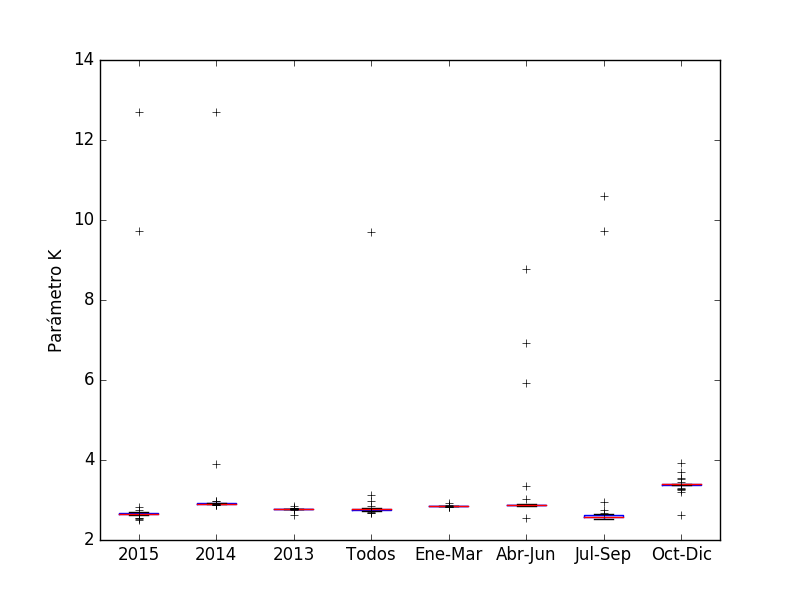
\includegraphics[width=0.75\textwidth]{figures/bp_param_K.png}
    \caption{Distribución de los parámetros K obtenidos en los distintos experimentos}
    \vspace{-.25cm}
    \caption*{Fuente: Elaboración Propia.}
    \label{fig:bp_param_K}
\end{figure}
\begin{figure}[ht!]
    \centering
    \captionsetup{justification=centering,margin=2cm}
    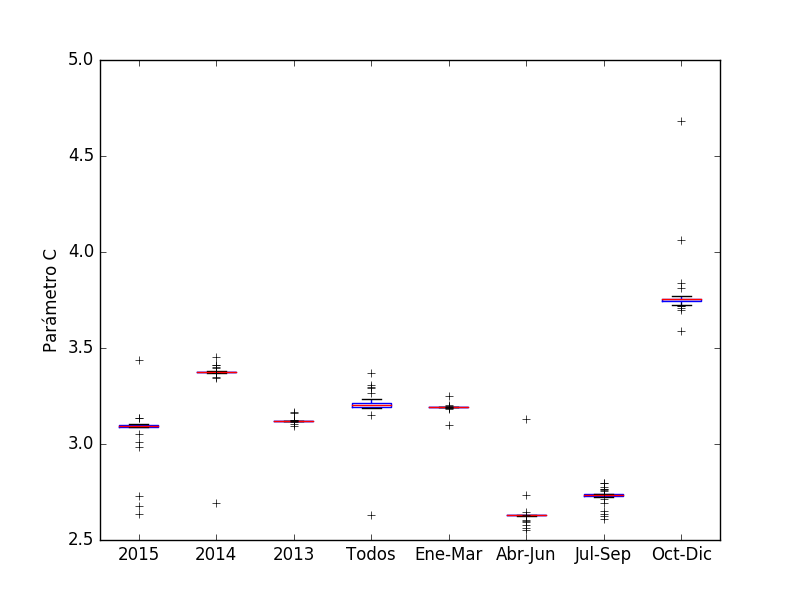
\includegraphics[width=0.75\textwidth]{figures/bp_param_C.png}
    \caption{Distribución de los parámetros C obtenidos en los distintos experimentos}
    \vspace{-.25cm}
    \caption*{Fuente: Elaboración Propia.}
    \label{fig:bp_param_C}
\end{figure}        

\newpage
\section{Conclusiones del capítulo}
En este capítulo se implementó la propuesta realizada en Carneiro et al. \cite{Carneiro15} para ajustar los parámetros de la distribución de Weibull a los datos de velocidad del viento en Valparaíso. Los resultados confirman que el método propuesto permite obtener soluciones de buena calidad, bajo el punto de vista de los test estadísticos aplicados (RMSE, r y RB), y los gráficos generados. Sin embargo, se debe tener en consideración que la distribución de Weibull representa el promedio diario de velocidades medidas del viento, detalle que no siempre se menciona en los trabajos que utilizan esta distribución, pero que se explican en algunos como en Fadare \cite{Fadare08}. Este modelo es útil para aplicaciones como la estimación del potencial eléctrico en determinada región.\\
Si se desea otra representación para las velocidades del viento, que permita representar velocidades predominantes, o una descripción más directa de los datos, como los representados en la Figura \ref{fig:pso_valpo_15_all_data}, se debe buscar otra distribución o una versión modificada de Weibull.\\
Los parámetros $k$ y $c$ obtenidos son similares en los distintos experimentos debido a la utilización del promedio diario de los datos lo cuál amortigua los valores extremos, variando principalmente por la cantidad de velocidades predominantes en el rango de tiempo considerado.\\
Finalmente, independiente de la semilla con la cual se ejecute el PSO, los resultados obtenidos son similares.